\section{Compact Object Abundance \Contact{Will}}
\label{sec:compact_objects}
\Contributors{William A.\ Dawson, Nathan Golovich, Simeon Bird, Yacine Ali-Ha\"imoud, Juan Garc\'ia-Bellido, Marc Moniez, Michael Medford, Robert Armstrong, Jessica Lu, Casey Lam}

MAssive Compact Halo Objects \citep[MACHOs;][]{1991ApJ...366..412G} have a long history as dark matter candidates \citep{1974ApJ...193L...1O, 1980ApJS...44...73B, 1981ApJ...243..140G, 1986ApJ...304....1P, Bellido:1996, Clesse:2015, Bird:2016, Clesse:2016}. 
Cosmological observations of the CMB, BAO, and deuterium abundances have shown that compact objects must be non-baryonic if they are to make up a majority of dark matter \citep[\eg][]{Ade:2015xua}. 
As described in \secref{machos}, this has led to the identification of primordial black holes (PBHs) as the most popular candidate for MACHO dark matter \citep{Bellido:1996}.
There are a number of astrophysical probes that constrain the PBH dark matter abundance over mass scales ranging from $10^{-17}-10^{15}\,M_\odot$ (\figref{macho_constraints}).
At the lowest masses ($M < 10^{-9}\Msun$), PBHs are constrained through the non-detection of PBH evaporation in the extragalactic gamma-ray background \citep[\eg,][]{0912.5297, 1604.05349}, non-detection of femto-lensing of gamma-ray bursts \citep[\eg,][]{1204.2056}, the rate of SN Type 1a \citep{1805.07381}, and neutron star capture \citep[\eg,][]{1301.4984}.
The landscape of intermediate-mass MACHOS ($10^{-11} \Msun < M < 10 \Msun$) is predominantly constrained by microlensing observations, which limit the monochromatic compact dark matter fraction to be $\lesssim 10\%$ over this mass range \citep[\eg,][]{2001ApJ...550L.169A, 2007A&A...469..387T, 2009MNRAS.397.1228W, 1509.04899, 1701.02151, Calcino:2018}.
At the high-mass end ($M \gtrsim 10^3\Msun$), PBH dark matter is subject to constraints from dynamical stability of wide binary stars \citep[\eg,][]{2009MNRAS.396L..11Q, 2004ApJ...601..311Y}, star clusters \citep[\eg,][]{2016ApJ...824L..31B, 1611.05052}, dwarf galaxies \citep{1704.01668}, and the Galactic disk \citep[\eg,][]{1985ApJ...299..633L, 1994ApJ...437..184X}.
Lyman-$\alpha$ observations disfavor PBHs with $M > 10^4\Msun$ based on an observed plateau in the Poisson term of the matter power spectrum \citep{astro-ph/0302035}.
Strong constraints have also been placed on the abundance of PBHs with mass $\gtrsim 1 \Msun$ using CMB anisotropies \citep{2008ApJ...680..829R}.
However, these constraints have been shown to be extremely model dependent and were relaxed substantially in subsequent studies \citep{2017PhRvD..95d3534A}.
%Several indirect constraints have been published that rule out most of the mass scales above the sensitivity of these microlensing surveys; however, these constraints rely on complex astrophysical assumptions.
This, in addition to recent direct observations by LIGO of mergers of $10-50 \Msun$ black holes, potentially with less spin than expected \citep{1602.03837, LIGOScientific:2018b, LIGOScientific:2018a},
has motivated a renewed interest in PBH dark matter with larger masses than have been so far constrained directly by microlensing.

\begin{figure}[t]
\centering
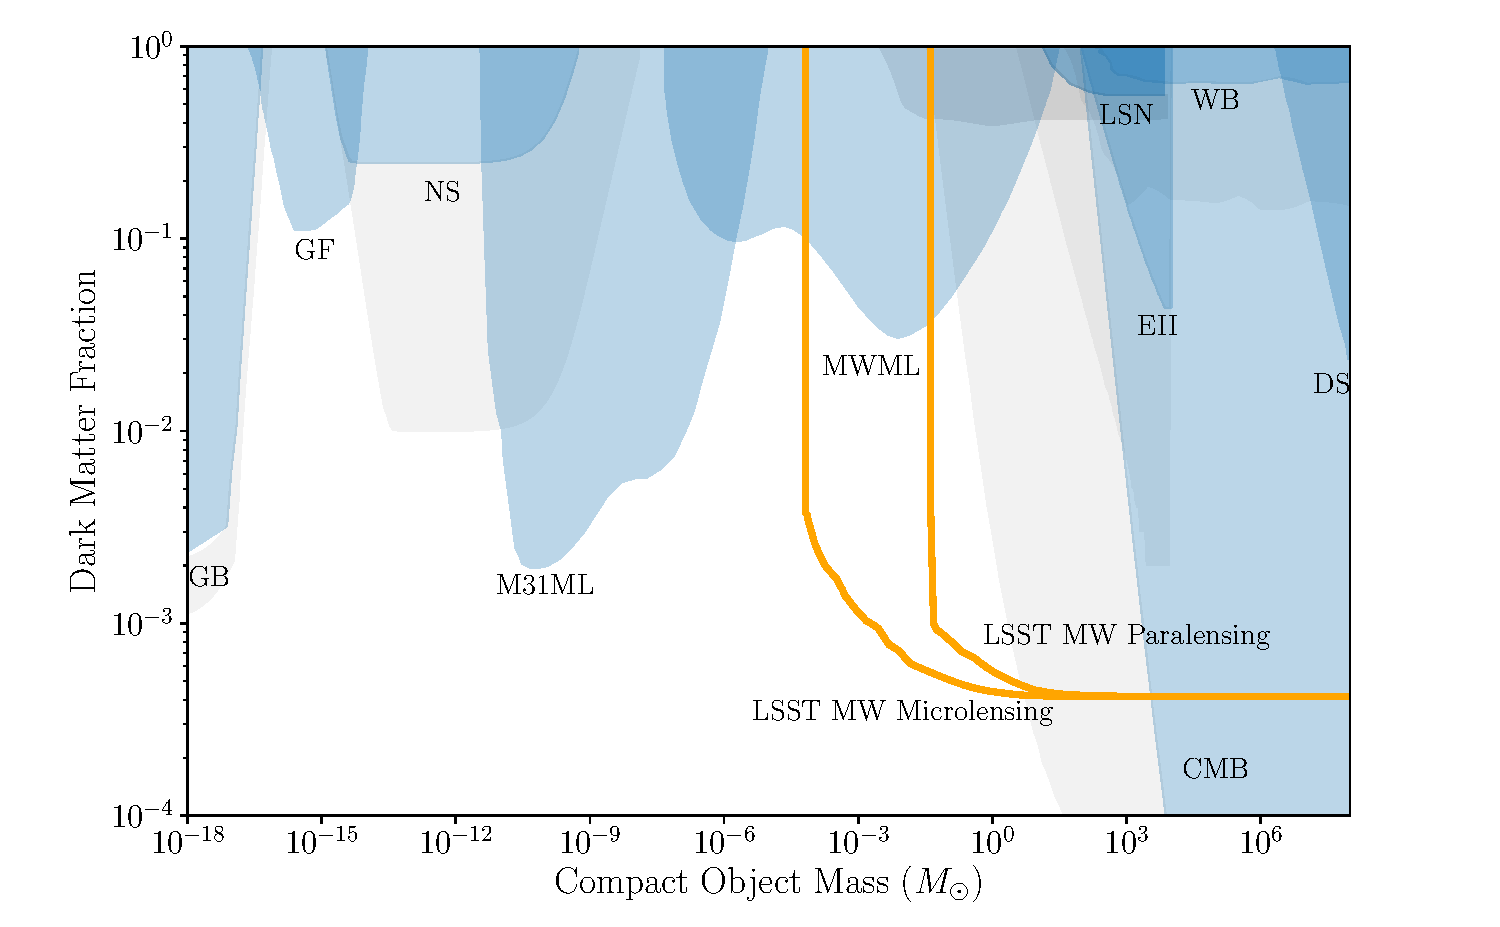
\includegraphics[width=0.75\textwidth]{macho_limits.pdf}
\caption{\label{fig:macho_constraints}
    Constraints on the maximal fraction of dark matter in compact objects from existing probes (blue and gray) and projections for LSST (gold).
    Existing constraints include: lack of extragalactic gamma-rays from PBH evaporation \citep[EGR;][]{0912.5297, 1604.05349}, gamma-ray femtolensing \citep[GF;][]{1204.2056}, neutron star capture \citep[NS][]{1301.4984}, M31 microlensing \citep[M31ML][]{1701.02151}, Milky Way microlensing \citep[MWML;][]{2007A&A...469..387T, 2001ApJ...550L.169A, 2009MNRAS.397.1228W}, lensing of supernovae \citep[LSN;][]{1712.02240,1712.06574}, Eridanus II and other dwarf-galaxy constraints \citep[EII;][]{2016ApJ...824L..31B, 1611.05052}, wide binary stars \citep[WB;][]{2009MNRAS.396L..11Q, 2004ApJ...601..311Y}, cosmic microwave background \citep[CMB;][]{2017PhRvD..95d3534A, 2008ApJ...680..829R}, and disk stability \citep[DS;][]{1985ApJ...299..633L, 1994ApJ...437..184X}.
    %To improve figure clarity we have not shown some astrophysical constraints where they are less sensitive than a presented constraint; see \citet{2016PhRvD..94h3504C} for a more complete review.
    There are a range of constraints for most astrophysical probes in the literature due to varying assumptions within a single work (EGR, NS, and EII) and reanalysis/disagreements between groups (WB, CMB).
    We present the most conservative constraints in blue and the most aggressive constraints in gray.
    %The LSST M31 microlensing projection is based on extrapolating HSC constraints \citep{1701.02151} assuming a 10-day mini-survey of M31 with a $12\second$ cadence between exposures.
    %% Such a survey is approximately 10 times longer with an order of magnitude faster cadence than the existing HSC survey.
    The projected LSST Milky Way (MW) microlensing and paralensing constraints are from a Monte Carlo analysis where lenses were injected into light curves based on LSST OpSim cadence simulations. 
    %% (see \url{https://github.com/lsstdarkmatter/dark-matter-paper/issues/8} for details).
    The paralensing constraint comes from assuming that only the secondary microlensing parallax signal is used for discovery, and not the primary heliocentric microlensing signal.
}
\end{figure}

In this section, we focus on the ability of LSST to directly detect signals of compact halo objects through precise, short ($\sim30\,$s) and long-duration ($\sim$ years) gravitational microlensing observations.
If scheduled optimally, the wide field-of-view, high cadence, and precise photometry of LSST \NEW{will provide sensitivity to the fraction of dark matter in compact objects down to} $\roughly 0.03\%$ for masses $>0.1\Msun$ (\figref{macho_constraints}).
We briefly mention that LSST will also probe PBHs by determining the rate of SN Type 1a, identifying candidate wide-binary star systems at greater distance than is possible with \Gaia, and through dedicated mini-surveys of high stellar density fields (similar to that performed with HSC by \citealt{1701.02151}).


\subsection{Microlensing}
\label{sec:microlensing}

Gravitational microlensing, the achromatic brightening and dimming of background stars due to the transit of a massive compact foreground object, can be used to directly detect and measure the properties of PBHs.
The idea of employing microlensing to search for compact objects in the Galactic halo was proposed by \citet{1986ApJ...304....1P}, and several photometric surveys commenced in the 1990's including MACHO \citep{1992ASPC...34..193A}, OGLE \citep{1992AcA....42..253U}, and EROS \citep{1993Msngr..72...20A}.
These collaborations provided the first \emph{direct} constraints on the compact nature of dark matter; however, they were limited by image quality, analysis techniques, and computational resources.
These limitations, combined with the $\roughly10$-year duration of these surveys, led to a loss of sensitivity at $M \gtrsim 1 \Msun$.
LSST can surpass this limitation by directly detecting events based purely on the parallactic component of the lensing signal (\figref{microlensing_cartoon}).
Furthermore, by supplementing the LSST survey with astrometric microlensing surveys using other telescopes (HST, Keck AO), LSST can break the lensing mass-geometry degeneracies and make precise measurements of individual black hole masses, thereby measuring the black hole mass spectrum in the Milky Way halo.
\NEW{If compact objects make up a significant fraction of dark matter, LSST will provide insight into the primordial perturbations and early universe equation of state, in the case of PBHs, or provide evidence that dark matter particle physics is complex enough to allow significant cooling channels. 
As dark matter with sufficient self-interactions to cool will also affect halo profiles, LSST will be well-placed to distinguish different models for the formation of novel compact objects.}
%Thus, if PBHs make up a significant fraction of dark matter, LSST will effectively measure their ``particle'' properties. 
%A precise measurement of the PBH mass spectrum will provide insight into the fundamental physics of the early universe.

\begin{figure}
\centering
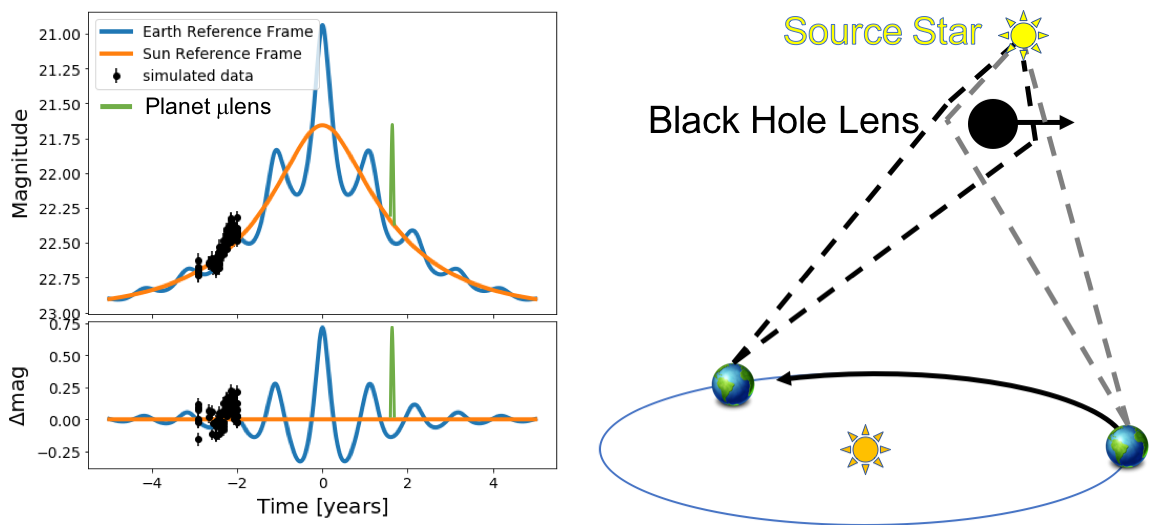
\includegraphics[width=0.7\columnwidth]{microlensing_cartoon.png}
\vspace{1em}
\caption{\label{fig:microlensing_cartoon}
    \emph{Left:} 
        The microlensing and paralensing signals for a $23 \magn$ source being lensed by a $50 \Msun$ black hole. 
        For events with an Einstein crossing time much less than a year ($\lesssim 1 \Msun$), the microlensing magnification will appear symmetric in time (orange curve).
        For microlensing events lasting on the order of a year or more ($\gtrsim 1 \Msun$), the lensing geometry changes due to parallax as Earth orbits the Sun.
        This paralensing signal has a period of a year, with the phase determined by the coordinates of the source star, making it robust to astrophysical systematics.
        %It is also possible to detect binary dark matter, and extend the mass range to planet mass compact dark matter, via the source passing through one of the gravitational lensing caustic curves formed by the binary lens.
        %The green curve on top of the heliocentric orange curve is representative of a typical planetary microlensing event caused by a caustic crossing.
        %While LSST can measure these events if lucky, we will rely on LSST to detect the heliocentric microlensing event and trigger targeted follow-up higher cadence observations to measure the planetary microlensing event.
        The black data points are representative of extending the LSST wide-fast-deep cadence into the Galactic plane. \WAD{Need to update this figure with the LSST WFD cadence.}
        \emph{Right:} 
        A cartoon diagram of paralensing. 
        For microlensing events lasting on the order of a year or more, the lensing geometry changes as Earth orbits the Sun, leading to a parallax effect.
        %\Contributors{Will D., PALS Collaboration}
    }
\end{figure}

\noindent \textbf{The Microlensing Signal}
%Gravitational microlensing occurs when a massive lens passes between a background source and an observer, causing the light from that source to pass through a warped space-time acting as a lens. \WAD{cite Wambsganss for a detailed review}

Gravitational microlensing results in two potentially observable features: (1) photometric microlensing, a temporary achromatic amplification of the brightness of the background source, and (2) astrometric microlensing, an apparent shift in the centroid position of the source.
The characteristic photometric signal of a simple point-source, point-lens (PSPL) model as observed from the center of the solar system is symmetric, achromatic, and has both a timescale and maximum amplification that depend on the mass of the lens.
LSST will observe billions of stellar sources in multiple filters over several years to enable the detection of thousands of microlensing events across a wide range of timescales and consequently a wide range of masses.
This simple PSPL model is complicated by astrophysical factors including the velocity distribution of sources and lenses, extinction due to Galactic dust, blending in dense stellar fields, and the shift in perspective resulting from viewing a microlensing event while the Earth revolves around the Sun.
Fortunately, these complications can be addressed and disentangled to arrive at the mass of the gravitational lens and a detection of dark matter via microlensing \citep{1405.3134,1509.04899}.

One particularly powerful feature for long-duration microlensing events results from the change in the geometric configuration of the source-lens-observer system as the Earth orbits the Sun (\figref{microlensing_cartoon}).
The change in viewing angle and distance results in a parallax effect that imposes a 1-year periodicity on top of an otherwise symmetric microlensing light curve.
This additional signal exists irrespective of the mass of the lens, providing an independent measurements of the distance of the lens and breaking the mass-distance degeneracy of a microlensing signal \citep[\eg,][]{1509.04899}.
This enables microlensing to directly constrain compact dark matter at much larger mass scales ($M \gtrsim 1\Msun$), where the duration of the event is $\gtrsim 1$ year. 
Based on Figure 3 from \citet{1509.04899}, we expect that LSST will be able to use paralensing to detect $10\Msun$ lenses out to a distance of $\roughly5 \kpc$.

Moreover, if primordial black holes are significantly clustered in the halo of our galaxy, forming pockets of hundreds of massive PBH, then one should expect to detect a few very-long-duration microlensing events, of order decades~\citep{Bellido:2017}. If one of the constituent PBH in the cluster happen to be directly along the line of sight of the magnified star then one would expect, on top of the smooth Paczynski curve, a sharp caustic associated with the Einstein-ring crossing time of the individual PBH within the cluster~\citep{Bellido:2018}.

%\ADW{What is the maximum distance for which the parallax signal is measureable?}


%\WAD{achromatic}
Gravitational lensing is achromatic, making the multiple filter observations of LSST a key advantage for distinguishing a microlensing signal from other astrophysical transient and variable objects.
The benefit derived from multi-filter observations will depend strongly on the selected LSST cadence. 
Microlensing signals are more easily extracted from frequent observations in fewer filters, as long as sources are observed in at least two colors. 


\noindent \textbf{Microlensing Systematics}

As with any empirical observation, microlensing measurements are subject to systematics that must be accounted for.
We briefly summarize these systematics and strategies for mitigating their effect.

\paragraph{Variable and binary stars:} Temporally variable objects are a potential source of false detections at all timescales. However, the microlensing signal can be distinguished because, modulo secondary ambiguous blending effects, it is achromatic. Most astrophysical variable and binary stars, by contrast, are associated with a temperature dependence and thus have chromatic variability. To leverage this fact, it is necessary for LSST to survey high-stellar-density fields in at least two bands. Furthermore, for microlensing events with durations $\gtrsim 1$ year, mimicking the annual parallax signal imprinted on the microlensing signal would require a binary or variable star with a period of exactly 1 year.

\paragraph{Blending:} Given the typical scale \WAD{give typical scale range for low and high mass} of the Einstein radius (the approximate region where a microlensing signal is detectable), the odds of a microlensing event along an arbitrary line of sight are $\roughly 10^{-7}$--$10^{-5.5}$ \citep[\eg,][]{2000ApJ...541..734A,2006ApJ...636..240S}.
Due to the low probability of a microlensing event, most observable microlensing events will be in dense stellar fields (e.g., the Galactic plane, Magellanic Clouds, M31), driving microlensing surveys to these regions.

These dense survey fields, coupled with LSST depth and ground based PSF with FWHM $\sim 0.7 \arcsec$ \citep{0805.2366}, lead to significant ambiguous blending (i.e., multiple objects within a single PSF).
Towards the Galactic center there are $\roughly 50$ stars within an LSST PSF, similarly there are $\roughly 15$ and $\roughly 5$ stars per PSF in the Galactic bulge and disk, respectively \citep{1806.06372}.
LSST can overcome much of the blending problem to detect variations in the brightness of stars, including the detection of microlensing lightcurves, through the process of difference imaging.
With difference imaging, reference images are built through the coaddition of multiple observation of the same fields, resulting in a deep image of the static sky. Reference images are then scaled and PSF-matched to individual observed science images and subtracted off, resulting in a difference image that only contains the signal that differs from the static sky. 

Difference imaging should reduce many of the systematic effects associated with blending. Follow-up high resolution imaging from space or gronud-based adaptive optics can mitigate most blending issues for detected microlensing events.
%; however, it will still be difficult to characterize the intrinsic source star baseline photometric properties. Crowding can also lead to a secondary chromatic signal with exactly the same duration/shape as the microlensing event, although with different amplitude. 
Blending systematics could also be mitigated through spectroscopic follow-up of microlensing events before and after crossing. Lensing by low-mass stars will alter the spectrum of the source, while PBH lensing will leave the spectrum unchanged.

\paragraph{Cadence:} The temporal cadence of LSST observations will be important for optimizing sensitivity to microlensing events. 
While high-mass PBHs should be accessible through relatively sparse observations distributed over the course of the year, smaller black holes require higher cadence observations.
\citep{1812.03137} suggest an observation strategy that includes a survey of the Galactic Bulge, Galactic Plane, and Magellanic Clouds with a reduced filter set at a cadence of 2 – 3 days. 
Observing the same region in at least two filters within the same night will allow tests of achromaticity.
\citet{1812.03139} suggest very high-cadence observations of the Magellanic Clouds (continuous 15s exposures), which should be sensitive to microlensing events from low-mass PBHs and scintillation light from invisible baryons \citep[\eg,][]{2003A&A...412..105M}.
The short readout time of the LSST Camera (2\,s) should allow for high-cadence observations of very short duration, subsolar mass PBHs, similar to the HSC observations of M31 \citep{1701.02151}.

\paragraph{Galaxy Model:} While microlensing can be detected independent of any detailed knowledge of Galactic structure, properly incorporating uncertainty in the Galactic dust, stellar velocity distributions, and dark matter halo model is essential to interpret the microlensing signal in the context of dark matter.
Significant improvements in our understanding of the Milky Way's dark matter halo have been made on this front since the first microlensing surveys \citep[\eg,][]{Calcino:2018}, and LSST will further improve these estimates (\secref{direct}).
In addition, systematic  microlensing measurements, especially when extended to the Galactic spiral arms, have the potential to strongly constrain the baryonic structure of the Galaxy in terms of mass density distribution and kinematical structure \citep[\eg,][]{Moniez:2017}.

%\paragraph{Binary vs isolated stars:} A potential systematic for the paralensing signal is binary star systems with approximately year-long periods. This is unlikely to be a significant systematic due to the low probability of having an achromatic binary system with a year long period. %\WAD{There was a researcher who did some of these studies for our microlensing group. Need to reference his work/arguments.} 

\noindent {\bf Projected Sensitivity}

%We estimate the projected sensitivity of an LSST survey optimized for the detection of microlensing signals from PBHs and present the results in \figref{macho_constraints}.
%The LSST M31 microlensing projection is based on extrapolating the \citet{1701.02151} by assuming a ten-day mini-survey of M31 with a 12 second cadence between exposures.
%Such a survey is approximately 10 times longer than that of \citet{1701.02151}, with an order of magnitude faster cadence.

We project the LSST Milky Way (MW) microlensing and paralensing sensitivity  from a Monte Carlo analysis of injected light curves based on LSST OpSim cadence simulations.
%\footnote{Details available in: \url{https://github.com/lsstdarkmatter/dark-matter-paper/issues/8}.}
We inject simulated microlensing signals onto the OpSim lightcurves for 200k PBH lenses in the mass range from $10^{-2}\Msun$ to $10^{8}\Msun$ distributed using a triangular density distribution, where $p(r = 0 \kpc) = 0$ and $p(r = 8\kpc) = 0.25$.
The sources are assumed to be $23\magn$ stars located at $8\kpc$ with measurement noise generated from the standard LSST photometric error model \citep{0805.2366}.
LSST is expected to detect $\roughly 10^{9}$ such stars, with an optical depth of $4.48 \times 10^{-6}$ \citep{2006ApJ...636..240S}.
The paralensing constraint comes from assuming that only the secondary microlensing parallax signal is used for discovery, and not the primary heliocentric microlensing signal.


